% !TEX program = xelatex
% 编译：xelatex report.tex （需 ctex 与 listings 宏包，TeX Live / MacTeX 自带）
\documentclass[a4paper,11pt]{article}

\usepackage[utf8]{inputenc}
\usepackage{ctex}                       % 中文支持
\usepackage[a4paper,margin=2.4cm]{geometry}
\usepackage{xcolor}
\usepackage{graphicx}
\usepackage{float}
\usepackage{listings}                   % 代码块
\usepackage{hyperref}
\usepackage{enumitem}
\usepackage{booktabs}
\usepackage{tabularx}
\usepackage{caption}
\usepackage{titlesec}

\hypersetup{
  colorlinks=true,
  linkcolor=[rgb]{0.05,0.35,0.55},
  urlcolor=[rgb]{0.10,0.45,0.70},
  citecolor=[rgb]{0.05,0.35,0.55},
}
\renewcommand{\refname}{参考项目}

%-------- 代码块样式 --------
\definecolor{codebg}{RGB}{248,249,250}
\definecolor{codeframe}{RGB}{208,211,215}
\definecolor{codekey}{RGB}{0,90,156}
\definecolor{codestr}{RGB}{106,115,125}
\definecolor{codecmt}{RGB}{110,125,110}

\lstdefinestyle{nicecode}{
  backgroundcolor=\color{codebg},
  basicstyle=\ttfamily\footnotesize,
  keywordstyle=\color{codekey}\bfseries,
  stringstyle=\color{codestr},
  commentstyle=\color{codecmt}\itshape,
  numbers=left,
  numberstyle=\tiny\color{gray!70},
  numbersep=8pt,
  frame=single,
  rulecolor=\color{codeframe},
  framesep=6pt,
  framerule=0.4pt,
  xleftmargin=16pt,
  breaklines=true,
  breakatwhitespace=true,
  showstringspaces=false,
  tabsize=4,
  columns=fullflexible,
  keepspaces=true,
  upquote=true,
  literate={'}{{\textquotesingle}}1,
}
\lstset{style=nicecode}

%-------- 行距与段落 --------
\linespread{1.25}
\setlength{\parskip}{4pt}
\emergencystretch=2em          % 允许额外拉伸，消除长 \texttt 词导致的 Overfull hbox

%-------- 标题样式 --------
\titleformat{\section}{\Large\bfseries\color[rgb]{0.05,0.35,0.55}}{\thesection}{0.6em}{}
\titleformat{\subsection}{\large\bfseries\color[rgb]{0.10,0.30,0.50}}{\thesubsection}{0.6em}{}

\begin{document}

\begin{center}
  
\includegraphics[width=0.85\textwidth]{../../assets/screenshots/title.png}
\end{center}
\vspace{6pt}

%================================================================
\begin{center}

演示视频与样例数据：

\url{https://disk.pku.edu.cn/link/AAAF21FBA1D86D4D1C96DDA3F3B7E7DFFD}
\end{center}

%================================================================
\section{程序功能介绍}

AutoReport 是一个跨平台的多 Agent 协作桌面应用，用于把“原始实验数据 + 参考资料”自动加工成一份可编译的 LaTeX 实验报告。用户只需准备好数据和参考文献，主控 Agent 会调度四个专职子 Agent 协同完成报告，并支持用户随时人工介入纠正方向，或主控 Agent 在发现问题时随时向子 Agent 反馈，因此并不一定严格按照流水线顺序执行。

\subsection{核心能力}

\begin{itemize}[leftmargin=1.4em,itemsep=2pt]
  \item \textbf{多 Agent 协作}：一个 Main Agent 负责统筹，四个子 Agent（数据分析 Data Analysis、绘图 Plotting、理论 Theory、报告 Report）各司其职。
  \item \textbf{目录权限隔离}：每个 Agent 只能写自己负责的目录（如绘图 Agent 只能写 \texttt{Plots/}），从机制上杜绝越权修改。
  \item \textbf{任务看板追踪}：用 waitlist / todolist 链式结构记录任务派发，子 Agent 完成后自动通知 Main Agent。
  \item \textbf{检查点回滚}：在消息节点自动打快照，可在时间线 UI 中回滚到任意历史状态。
  \item \textbf{随时人工介入}：用户可在任意时刻向任意 Agent 发消息，纠正方向或补充要求。
\end{itemize}

\subsection{交互与界面}

GUI 采用 VSCode 风格\cite{vscode}，三栏布局：左侧文件树（6 个固定目录）、中间预览/编辑、右侧单个 Agent 面板。该面板顶部有一个下拉选择器，用于在 Main / Data Analysis / Plotting / Theory / Report 五个 Agent 之间切换；左侧选中目录不再联动切换 Agent（目录导航与 Agent 切换已解耦）。支持流式输出、Markdown 渲染、工具调用分组展示、\texttt{@} 文件引用与斜杠命令（\texttt{/compact}、\texttt{/new}、\texttt{/init} 等）。

启动时先进入项目选择窗口，可打开已有实验文件夹、新建项目、配置 API 或从最近项目恢复：

\begin{figure}[H]
  \centering
  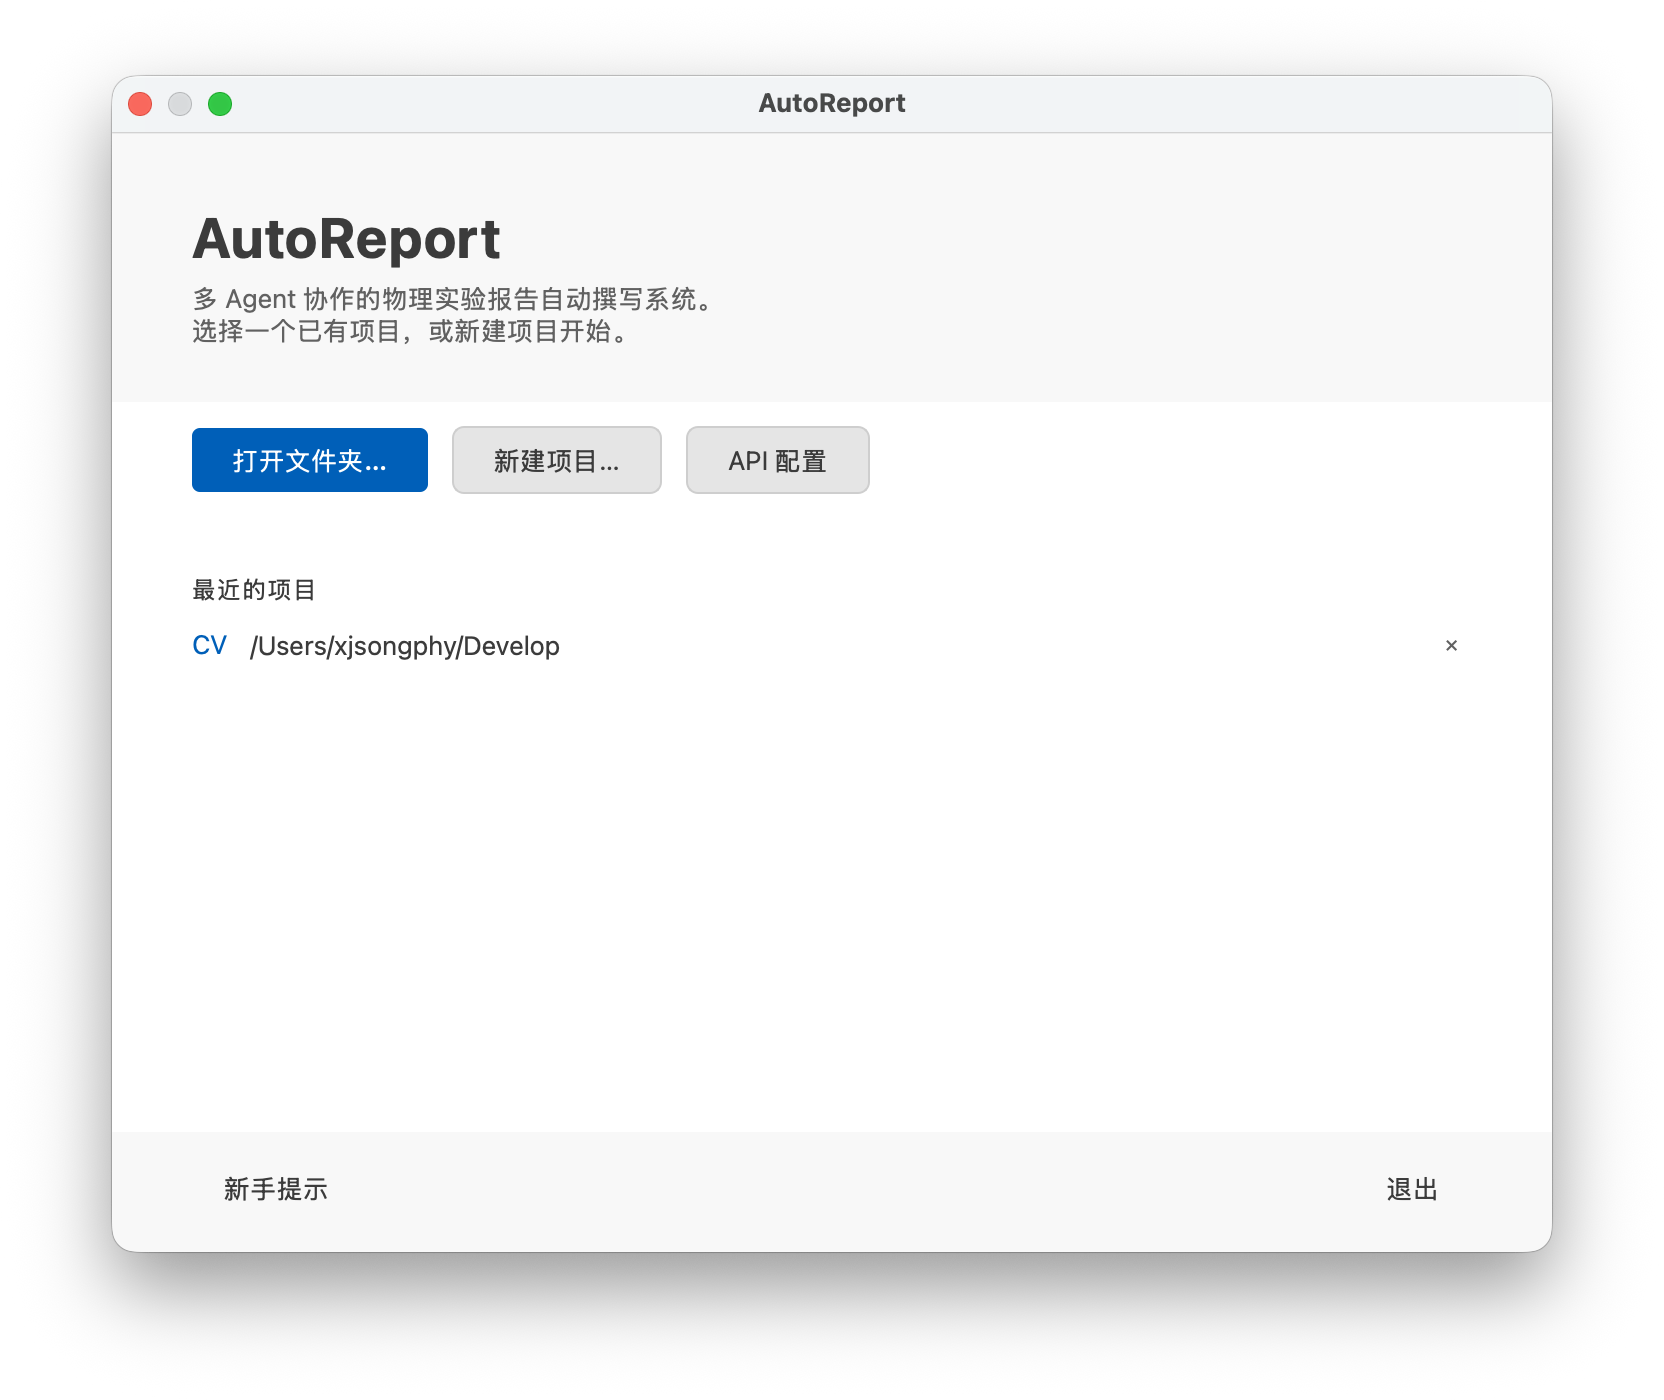
\includegraphics[width=0.7\textwidth]{../../assets/screenshots/start-window.png}
  \caption{AutoReport 启动窗口}
\end{figure}

进入主工作区后，文件树、文档预览、Agent 聊天时间线同屏可见，用户可一边查看生成的 LaTeX/PDF，一边与 Agent 团队交互：

\begin{figure}[H]
  \centering
  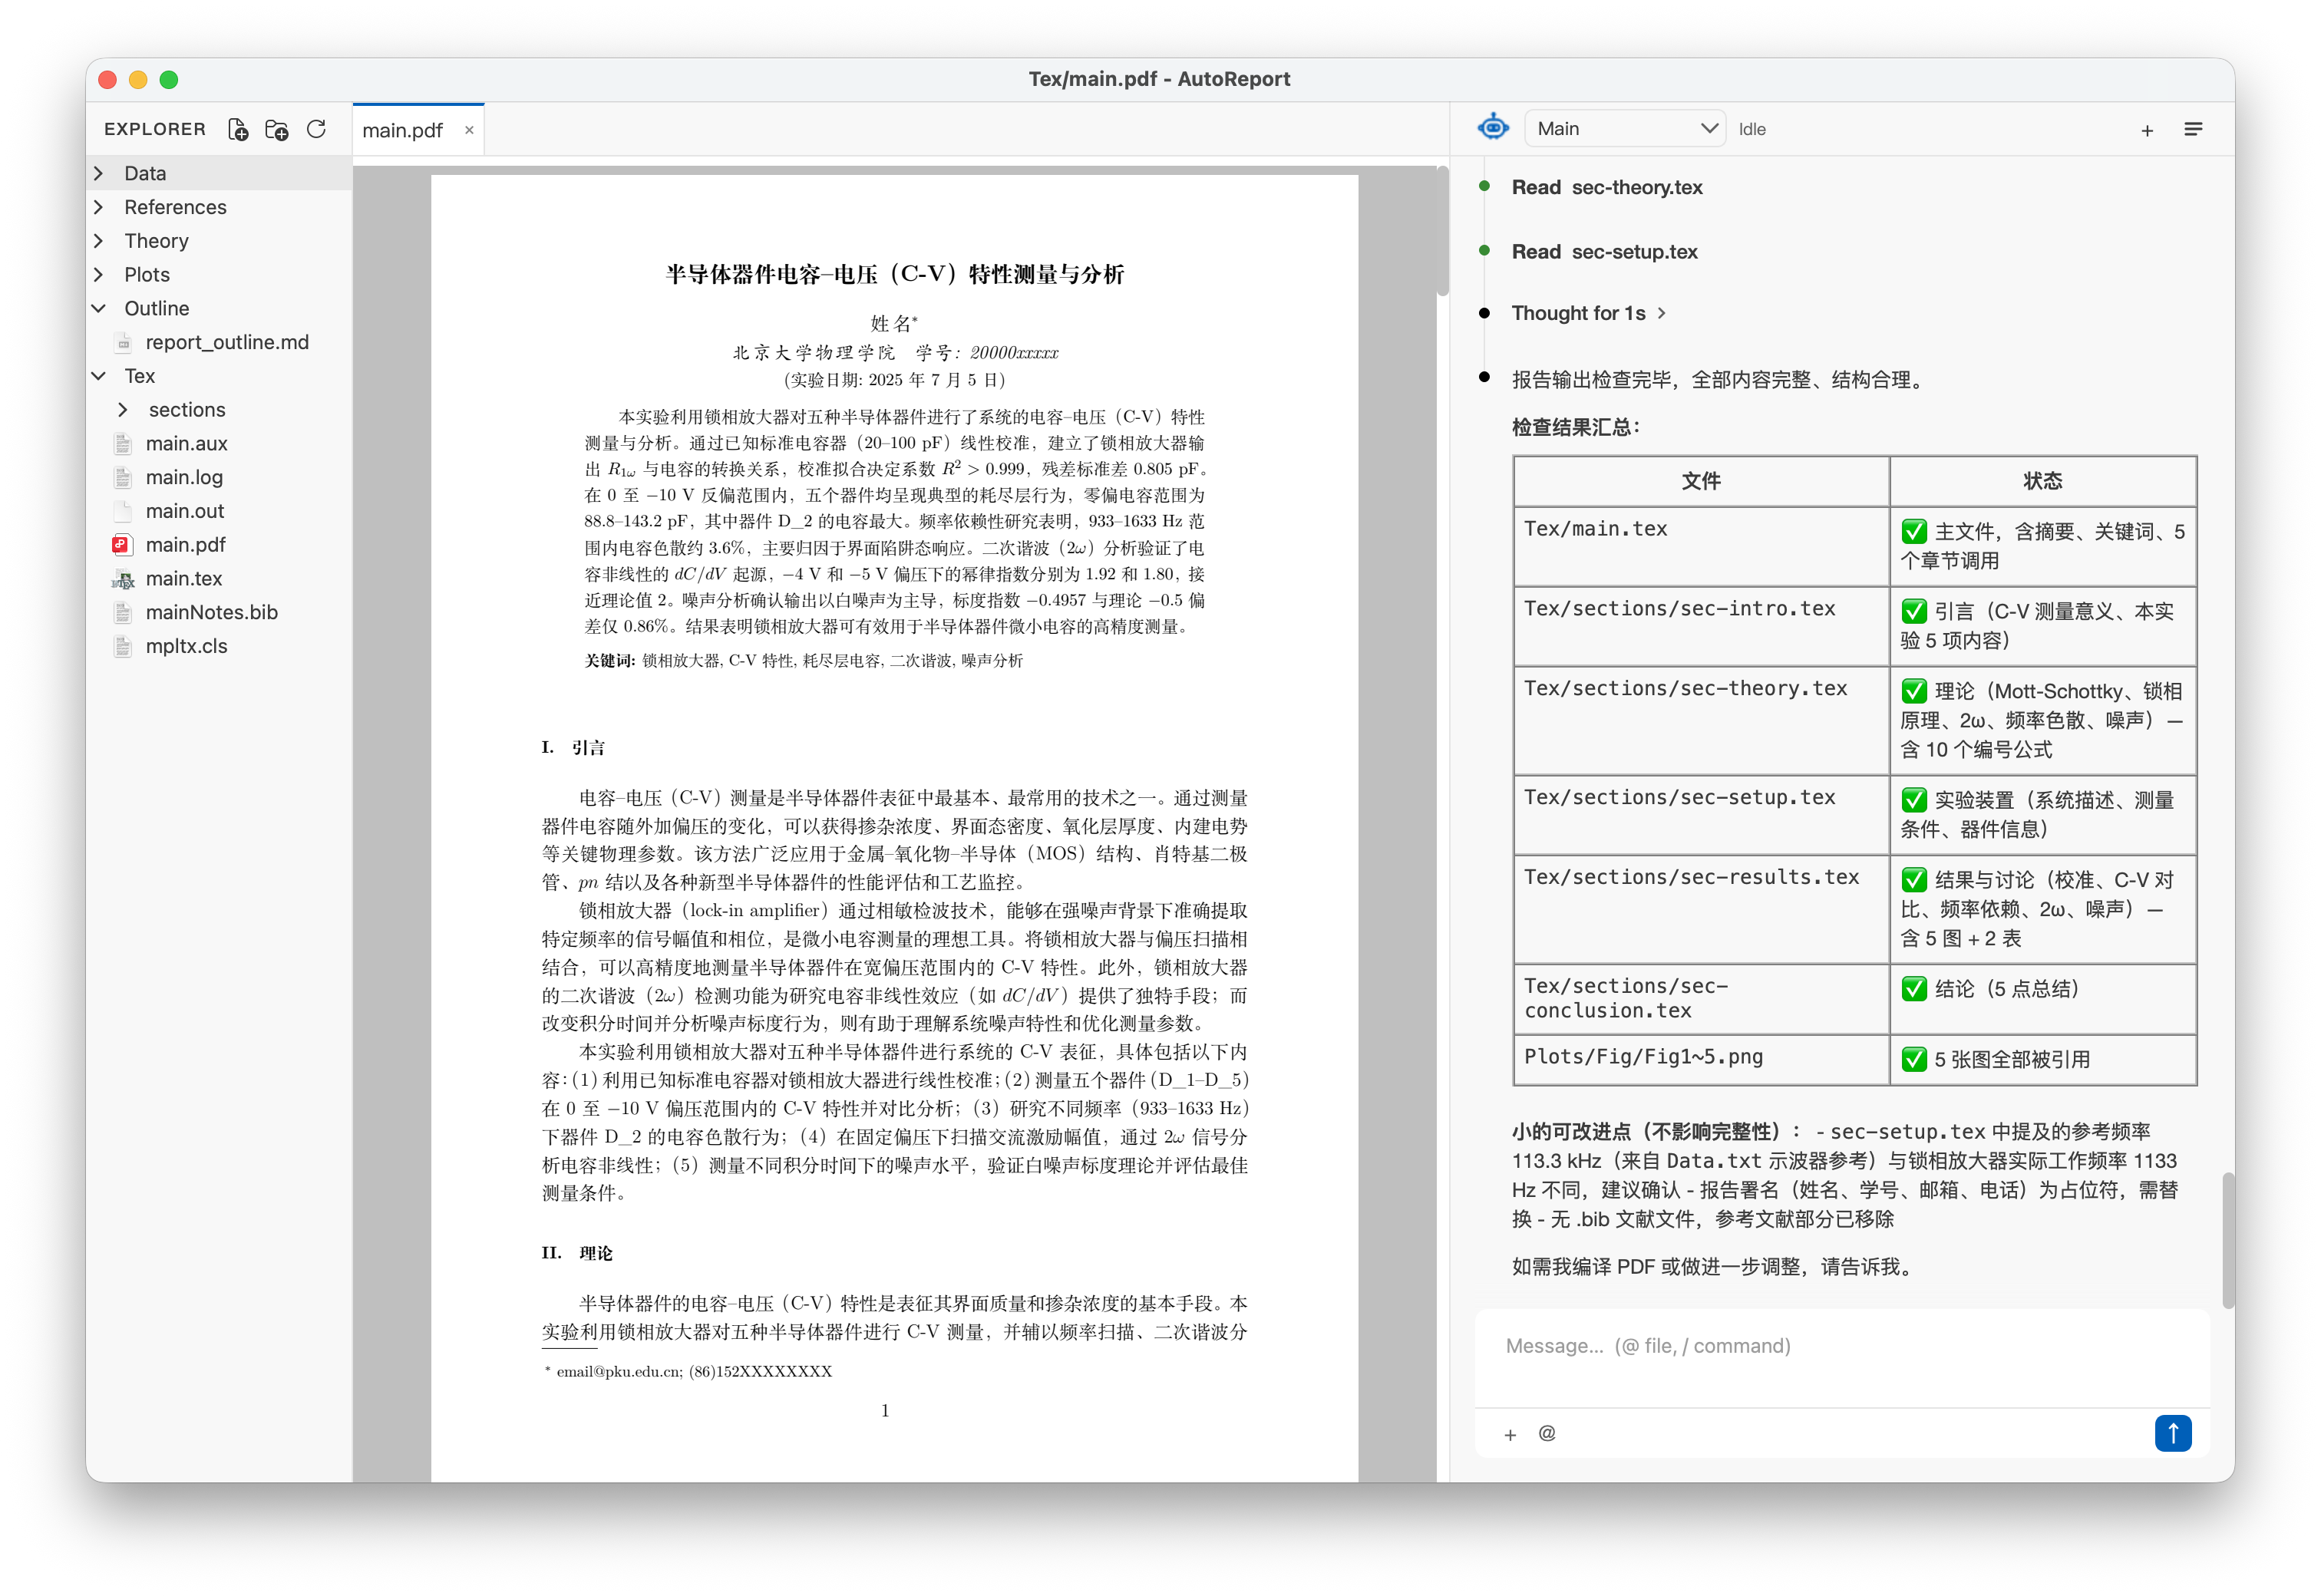
\includegraphics[width=0.8\textwidth]{../../assets/screenshots/main-window.png}
  \caption{AutoReport 主工作区（三栏布局）}
\end{figure}

\subsection{LLM 集成}

AutoReport 支持 Anthropic、OpenAI、DeepSeek 等多家 Provider；可从 cc-switch\cite{ccswitch} 同步 50+ 个 Provider 预设；Agent Prompt 由 \texttt{PromptLoader} 加载（每个 Agent 一个完整 Markdown 文件，加载后缓存），并内置上下文自动压缩。Provider 预设、当前 Provider、API key、base URL 与默认模型在配置对话框中统一管理：

\begin{figure}[H]
  \centering
  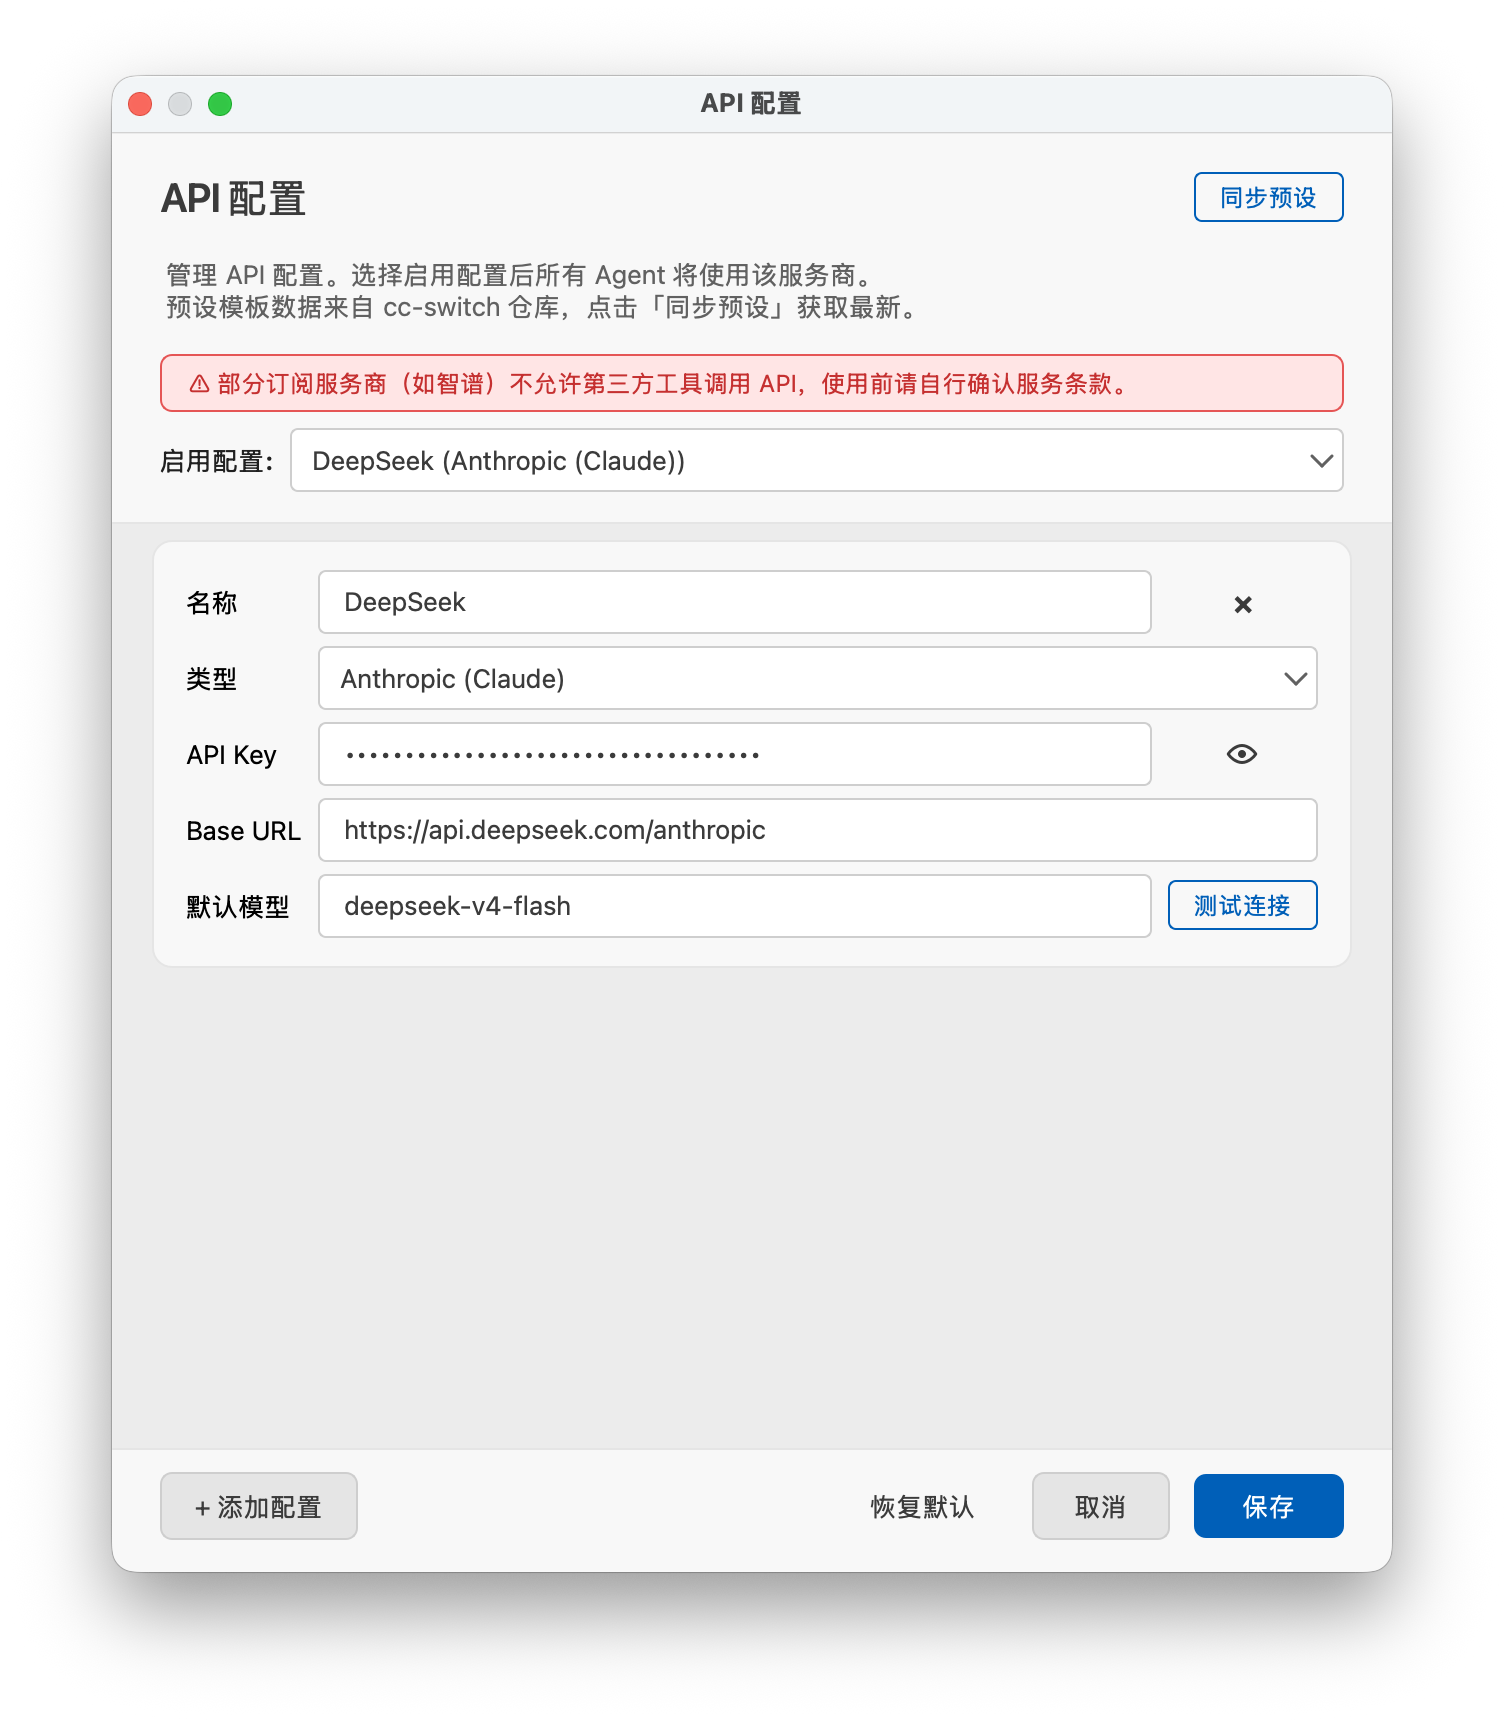
\includegraphics[width=0.85\textwidth]{../../assets/screenshots/configuration-window.png}
  \caption{AutoReport API 配置对话框}
\end{figure}

\subsection{典型工作流}

\begin{figure}[H]
  \centering
  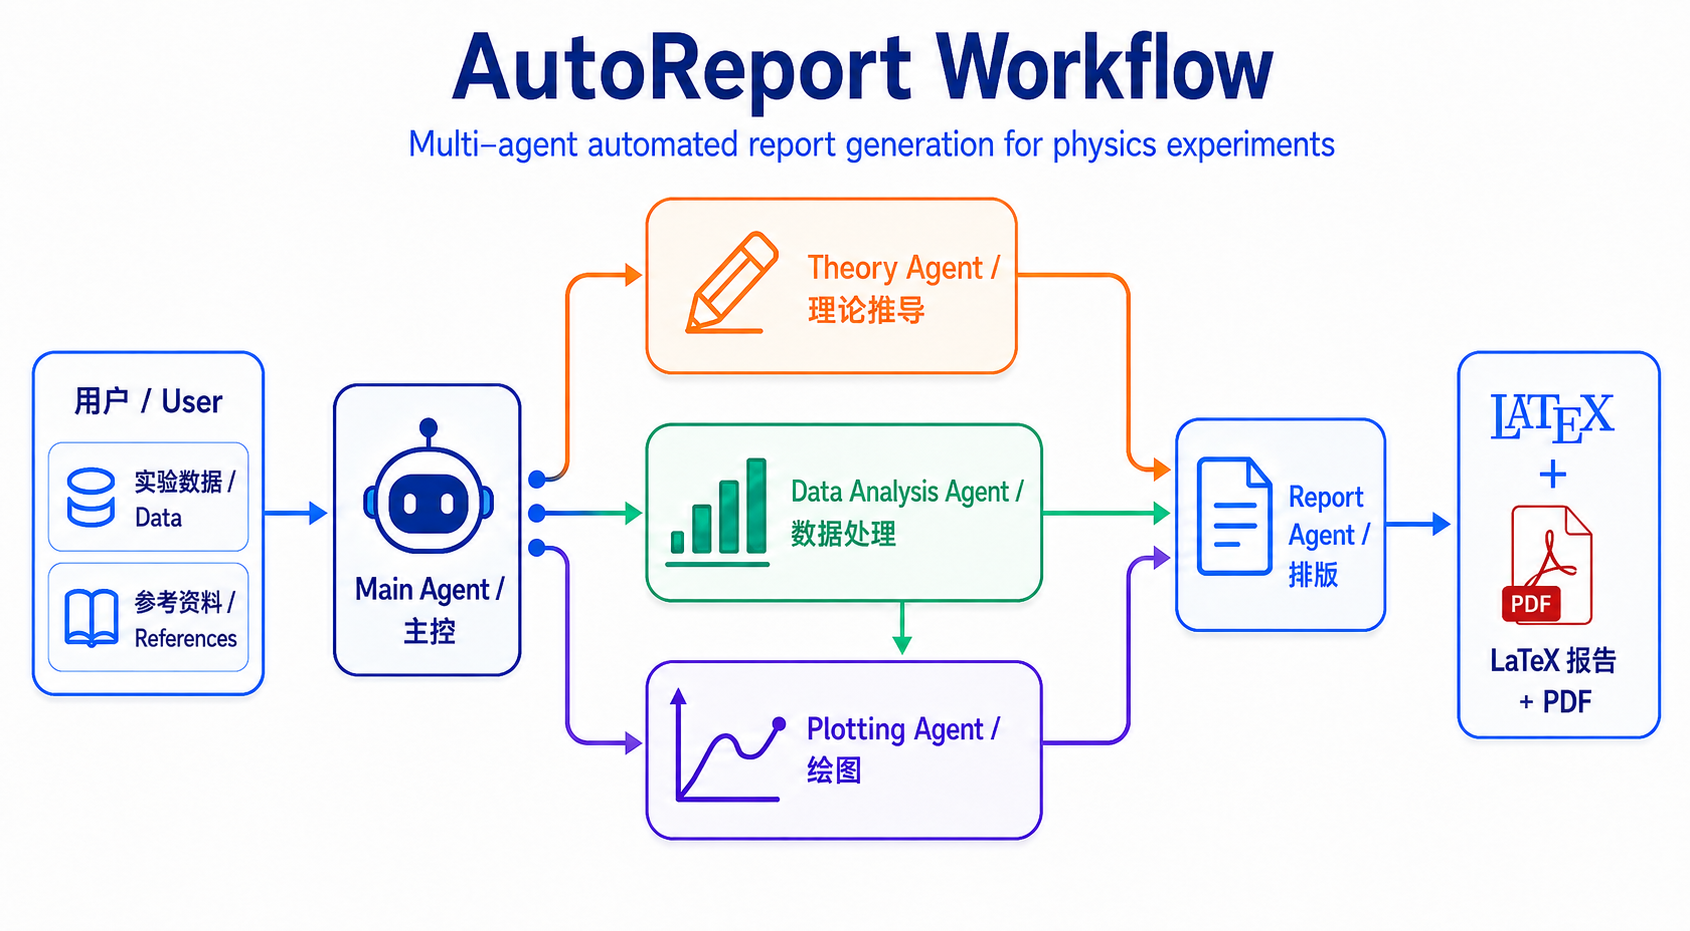
\includegraphics[width=0.95\textwidth]{../../assets/screenshots/workflow.png}
  \caption{多 Agent 协作流程实际运行示例}
\end{figure}

Main Agent 解析需求后把子任务派发给对应子 Agent，子 Agent 在各自目录中产出文件，最后由 Report Agent 使用内置 LaTeX 报告模板（基于 PKUMpLtX\cite{pkumplt} 北大近代物理实验模板，revtex4-2 格式）汇总编译为 PDF。整个过程中用户可随时介入。

%================================================================
\section{项目各模块与类设计细节}

项目用 Python 3.12 开发，\texttt{uv} 管理依赖，\texttt{hatchling} 打包，PyQt6 构建 GUI，直接调用 \texttt{anthropic} 与 \texttt{openai} 原生 SDK（不经过 LangChain 等抽象框架），配置层用 Pydantic。源码约 2.8 万行，整体目录如下：

\begin{lstlisting}[language={},basicstyle=\ttfamily\footnotesize]
autoreport/
+- app.py              # 入口：CLI 解析、配置/项目对话框、主窗口启动
+- config/             # Pydantic 配置 schema、YAML 加载、API key 校验
+- core/
|   +- loops/          # Agent 运行时：manager / agent_loop / bus
|   +- providers/      # LLM Provider 抽象：factory / base / anthropic / openai
|   +- tools/          # 工具系统：registry + 各类具体工具
|   +- checkpoints.py  # 操作日志式检查点与回滚
|   +- prompts/        # Agent Prompt 加载（完整指令 + 缓存）
|   +- file_search.py  # @ 引用的模糊文件搜索
+- gui/                # PyQt6 界面：main_window + widgets
+- interfaces/         # GUI <-> 后端 协议与消息类型
+- templates/          # 内置 Agent Prompt 与报告模板
\end{lstlisting}

下面按子系统说明大致逻辑、所用库与关键控件，必要时引用源码。

\subsection{配置层（\texttt{config/}）}

\texttt{schema.py} 用 Pydantic 定义 \texttt{Settings} 及各 Agent 的 \texttt{AgentDefaults}（温度、上下文窗口、最大 token 等）；\texttt{manager.py} 负责从 \texttt{autoreport.config.yaml} 读取配置并在缺失时回退到环境变量；\texttt{presets.py} 维护从 cc-switch 同步来的 Provider 预设。这一层的设计借鉴了参考项目 DeepCode\cite{deepcode} 的“YAML 密钥 + 环境变量回退”思路。

\subsection{Agent 运行时（\texttt{core/loops/}）}

这是整个系统的心脏，由三个类协作。

\textbf{MessageBus} 是基于 \texttt{asyncio.Queue} 的发布/订阅消息总线。组件按消息类型订阅，总线把消息派发给所有匹配的回调，它是 Main Agent 与子 Agent 之间异步通信的唯一通道：

\begin{lstlisting}[language=Python]
class MessageBus:
    async def publish(self, message: Message) -> None:
        await self._queue.put(message)

    async def process_queue(self) -> None:
        while not self._shutdown:
            message = await asyncio.wait_for(
                self._queue.get(), timeout=1.0
            )
            await self._notify_subscribers(message)
\end{lstlisting}

\textbf{LoopManager} 管理所有 AgentLoop 的生命周期，并为每个 Agent 构造\textbf{工具隔离的} \texttt{ToolRegistry}——根据该 Agent 的写权限注册不同的工具子集，使 Agent 在机制上无法越权写文件。它还持有 \texttt{CheckpointManager}、\texttt{TaskBoard}、\texttt{ManifestManager} 等共享组件。

\textbf{AgentLoop} 是单个 Agent 的处理引擎，核心是“LLM 调用 $\rightarrow$ 工具执行”的最大迭代循环。其设计借鉴参考项目 nanobot\cite{nanobot} 的 AgentLoop 架构。关键逻辑包括：

\begin{itemize}[leftmargin=1.4em,itemsep=2pt]
  \item \textbf{Prompt 加载}：由 \texttt{PromptLoader} 读取 \texttt{templates/agents/} 下每个 Agent 的完整 Markdown 指令（含共享的 \texttt{Common.md}），加载后缓存复用。
  \item \textbf{流式调用}：通过 \texttt{llm\_provider.chat\_stream} 边生成边把 delta 推送到 UI。
  \item \textbf{工具调用处理}：当 LLM 返回 \texttt{tool\_calls} 时，交给 \texttt{\_handle\_tool\_calls} 在注册表中查表执行，结果回填进对话历史，再次调用 LLM。
  \item \textbf{上下文自动压缩}：\texttt{\_trim\_messages\_to\_budget} 在每轮调用前估算 token 数，超预算时裁剪历史，并清理裁剪边界产生的孤儿消息（如失去配对的 \texttt{tool\_result}），避免触发 API 报错。
  \item \textbf{响应守卫}：子 Agent 在结束一个由 Main 派发的回合前必须调用 \texttt{respond} 工具汇报结果（\texttt{\_enforce\_report\_guard}），Main Agent 不允许在持有 BLOCKED 任务时进入 IDLE（\texttt{\_enforce\_main\_blocked\_guard}），这两层保证流水线不会“卡死或静默退出”。
\end{itemize}

\subsection{Provider 抽象（\texttt{core/providers/}）}

\texttt{base.py} 定义与具体厂商无关的数据类 \texttt{Message}、\texttt{LLMResponse}、\texttt{LLMStreamChunk} 及抽象基类 \texttt{LLMProvider}；\texttt{factory.py} 的 \texttt{ProviderFactory} 按 \texttt{provider\_type} 实例化对应实现——\texttt{anthropic} 走 \texttt{AnthropicProvider}，其余（OpenAI、DeepSeek、Google、OpenRouter 等 OpenAI 兼容接口）统一走 \texttt{OpenAICompatProvider}。两套 Provider 把内部的统一 \texttt{Message} 结构翻译成各自 SDK 要求的格式（Anthropic 的 \texttt{tool\_use} / \texttt{tool\_result} content block，OpenAI 的 \texttt{tool\_calls} 字段）。这部分的多 Provider 思路与错误处理同样参考了 DeepCode\cite{deepcode}，AgentLoop 主体与工具定义风格则参考了 nanobot\cite{nanobot}。

\subsection{工具系统（\texttt{core/tools/}）}

\textbf{ToolRegistry} 的设计是\textbf{从函数签名自动生成 JSON Schema}：每个 \texttt{Tool} 子类只需写 \texttt{name}、\texttt{description} 和 \texttt{\_\_call\_\_} 的类型注解，注册表用 \texttt{inspect} + \texttt{get\_type\_hints} 反射出 \texttt{input\_schema}，组装成 LLM 的 function calling，新增工具时几乎零样板代码。

具体工具按职能分层：

\begin{itemize}[leftmargin=1.4em,itemsep=2pt]
  \item \textbf{通用工具}：\texttt{ReadTool}（按行范围读）、\texttt{ApplyPatchTool} / \texttt{WriteFileTool}（写文件并自动备份）、\texttt{ExecTool}（受白名单约束的 shell 执行）。
  \item \textbf{专职工具}：数据分析 Agent 有 CSV/Excel 读取与 \texttt{python\_exec}；绘图 Agent 有 matplotlib 执行与图片管理；报告 Agent 有 LaTeX 编译（xelatex/lualatex）和经 MinerU\cite{mineru} 服务解析 PDF 的 \texttt{PDFParseTool}。
  \item \textbf{协作工具}：\texttt{SendToAgentTool}（派发任务）、\texttt{RespondTool}（子 Agent 汇报）、\texttt{ManageTasksTool}（任务看板）。
  \item \textbf{技能（Skill）工具}：\texttt{LoadSkillTool} 从 \texttt{external/skills/} 加载独立的 Markdown 技能文件（如 \texttt{latex-compile}、\texttt{experiment-report-writer}），这些文件由 \texttt{preset\_sync.py} 从自维护的 skills 仓库\cite{skills} 同步，使 Agent 在不污染主提示词的前提下按需获得 LaTeX 编译、实验报告撰写等领域能力。
\end{itemize}

\texttt{ExecTool} 采用\textbf{白名单 + 路径安全校验}：命令基础名必须在 \texttt{ALLOWED\_COMMANDS} 白名单内，再额外拦截对内部元数据目录的访问、对系统目录（\texttt{/}、\texttt{/usr} 等）的删除以及 \texttt{..} 路径穿越，作为命令执行的安全沙箱。

\subsection{检查点与回滚（\texttt{core/checkpoints.py}）}

采用 codex\cite{codex} 风格的\textbf{操作日志}而非完整快照 + diff 链：每当工具改动文件时，把这次改动记录成可逆的 \texttt{FileOperation}，回滚就是逆序回放这些操作。这样记录精确、无 diff 累积误差，且因为 \texttt{apply\_patch} 只处理文本，二进制文件（PDF、图片）天然不会被误回滚。每个 Agent 维护独立的时间线，存于 \texttt{.checkpoints/\{agent\_type\}/}。

\subsection{GUI 层（\texttt{gui/}）}

PyQt6 实现，\texttt{MainWindow} 组装三栏布局。关键控件包括：

\begin{itemize}[leftmargin=1.4em,itemsep=2pt]
  \item \textbf{FileTreeWidget}：左侧 6 个固定目录（Data、References、Theory、Plots、Outline、Tex）的文件树，基于 \texttt{QTreeWidget}，支持目录内增删、拖拽、\texttt{Cmd/Ctrl} 多选。
  \item \textbf{PreviewWidget}：中间内容视图，按左侧选中目录切换渲染方式（表格 / 文本预览 / 代码 + 图片 / TeX + PDF）。TeX 与代码高亮使用 \texttt{pyqt6-qscintilla}（Scintilla 编辑器控件）。
  \item \textbf{AgentPanel}：右侧 Agent 面板，顶部 \texttt{NoWheelComboBox} 选择器切换当前 Agent，下方含时间线（\texttt{Timeline}）与聊天区。其整体外观与交互（气泡式消息、工具调用分组折叠、流式输出、\texttt{@} 引用与斜杠命令补全）参考了 Claude Code\cite{claudecode} 的 IDE 插件界面。
  \item \textbf{MessageRow / ToolCallGroup}：气泡式消息展示，工具调用分组折叠，Markdown 用 \texttt{markdown} 库渲染。
  \item \textbf{ChatInput}：支持 \texttt{@} 触发模糊文件搜索并插入引用，斜杠命令弹出补全。
\end{itemize}

界面统一主题颜色由 \texttt{theme.py} 集中管理，并兼容深色模式。

\subsection{接口层（\texttt{interfaces/types.py}）}

用 Pydantic \texttt{BaseModel} 定义所有 GUI 与后端之间的消息类型（\texttt{UserMessage}、\texttt{AgentResponse}、\texttt{ToolCallMessage}、\texttt{ReportMessage}、\texttt{SystemNotice} 等）与枚举（\texttt{AgentType}、\texttt{AgentStatus}、\texttt{TaskStatus}）。\texttt{MessageType} 区分 GUI$\rightarrow$后端与后端$\rightarrow$GUI 两个方向。统一类型保证消息在总线与 UI 之间传递时强类型、可序列化。

%================================================================
\section{小组成员分工}

\begin{table}[H]
\centering
\renewcommand{\arraystretch}{1.35}
\begin{tabularx}{\textwidth}{@{}p{2.2cm}X@{}}
\toprule
\textbf{成员} & \textbf{主要职责} \\
\midrule
宋昕杰 & 项目主体开发。负责项目框架初步搭建、GUI 大部分模块（主窗口、文件树、预览、Agent 面板、消息气泡、主题系统、配置/项目对话框）、核心运行时（AgentLoop / LoopManager / MessageBus）、工具系统、Provider 抽象、检查点系统、文件搜索，以及大量测试与 Bug 修复。 \\
宋敬哲 & 新用户教程系统、提示词优化、画图质量管控（脚本校验 + Agent 自查协议）、双轨日志系统、MAIN 权限收窄。 \\
郑志恒 & File 工具、Provider 层 Bug 修复：Anthropic 流式响应中 \texttt{thinking\_delta} 的保留、防止向 Anthropic API 发送空 content 消息。 \\
\bottomrule
\end{tabularx}
\end{table}

%================================================================
\section{项目总结与反思}

在 Agent 时代，多 Agent 协作的桌面应用是一个有趣的尝试。通过这个项目，我们更好地理解了 Agent 背后的相关机制、原理以及设计原则，并且在主流工具之外实现了 Manifest 工具和任务派发工具。我们在查阅 Codex\cite{codex} 的相关设计时，了解到提示词的设计应当相信 LLM 的能力，尽量减少对 LLM 的约束，避免过度设计。我们基于此原则，在达到实验报告写作目标的基础上，尽量精简了提示词。

开发过程中，Coding Agent 的使用确实加快了开发进程，但效率提升导致同时维护多个功能或修复多个 Bug 时，PR 不及时提交、变动过大、难以审阅。同时我们对 GitHub 协作的使用也有了更深的理解，尤其是 PR 的使用和分支管理，比如 PR 的互相审查以及避免直接改动他人的分支。

带有 GUI 的项目开发难度明显高于纯代码项目，尤其是 PyQt6 的相关显示部分。Coding Agent 的多模态能力还略有欠缺，需要人工多次打磨相关代码设计，才能得到功能良好的代码。

\begin{thebibliography}{9}
\setlength{\itemsep}{2pt}

\bibitem{vscode} Microsoft. \textbf{Visual Studio Code / Code - OSS}. GitHub 仓库. \url{https://github.com/microsoft/vscode}

\bibitem{ccswitch} farion1231. \textbf{CC Switch: All-in-One Manager for Claude Code, Codex, Gemini CLI, OpenCode, OpenClaw and Hermes Agent}. GitHub 仓库. \url{https://github.com/farion1231/cc-switch}

\bibitem{pkumplt} CastleStar14654. \textbf{PKUMpLtX: 北京大学近代物理实验 LaTeX 报告模板（基于 revtex4-2）}. GitHub 仓库. \url{https://github.com/CastleStar14654/PKUMpLtX}

\bibitem{deepcode} Data Intelligence Lab @ HKU (HKUDS). \textbf{DeepCode: Open Agentic Coding}. GitHub 仓库. \url{https://github.com/HKUDS/DeepCode}

\bibitem{nanobot} Data Intelligence Lab @ HKU (HKUDS). \textbf{nanobot: Lightweight, Open-Source Personal AI Agent}. GitHub 仓库. \url{https://github.com/HKUDS/nanobot}

\bibitem{mineru} OpenDataLab. \textbf{MinerU: A Tool for Extracting Markdown and JSON from PDFs and Office Documents}. GitHub 仓库. \url{https://github.com/opendatalab/MinerU}

\bibitem{skills} xjsongphy. \textbf{skills: Agent Skill Files (latex-compile, experiment-report-writer, \ldots), synced via \texttt{preset\_sync} into \texttt{external/skills/}}. GitHub 仓库. \url{https://github.com/xjsongphy/skills}

\bibitem{codex} OpenAI. \textbf{Codex CLI: Lightweight Coding Agent That Runs in the Terminal}. GitHub 仓库. \url{https://github.com/openai/codex}

\bibitem{claudecode} Anthropic. \textbf{Claude Code: Agentic Coding System}. 产品文档. \url{https://claude.com/claude-code}

\end{thebibliography}

\end{document}
